\subsection{Actividad 8}
Verificar si es posible compensar en discreto el sistema
servomotor de posición con un controlador proporcional para que el
sistema en bucle cerrado cumpla las especificaciones de
sobreoscilación $< 5 \%$ y tiempo de establecimiento $t_{\text{est}} < 0.3 s$. y
error nulo ante consigna escalón unitaria, graficando la respuesta
escalón.

\begin{tcolorbox}[sharp corners, colframe=bluebox, title= Compensador
  proporcional en tiempo discreto.]
  $>>>$ rltool(Gposicionz)\\
  \vspace*{0.35em}
  \mkanscode{
\begin{figure}[H]
  \centering
  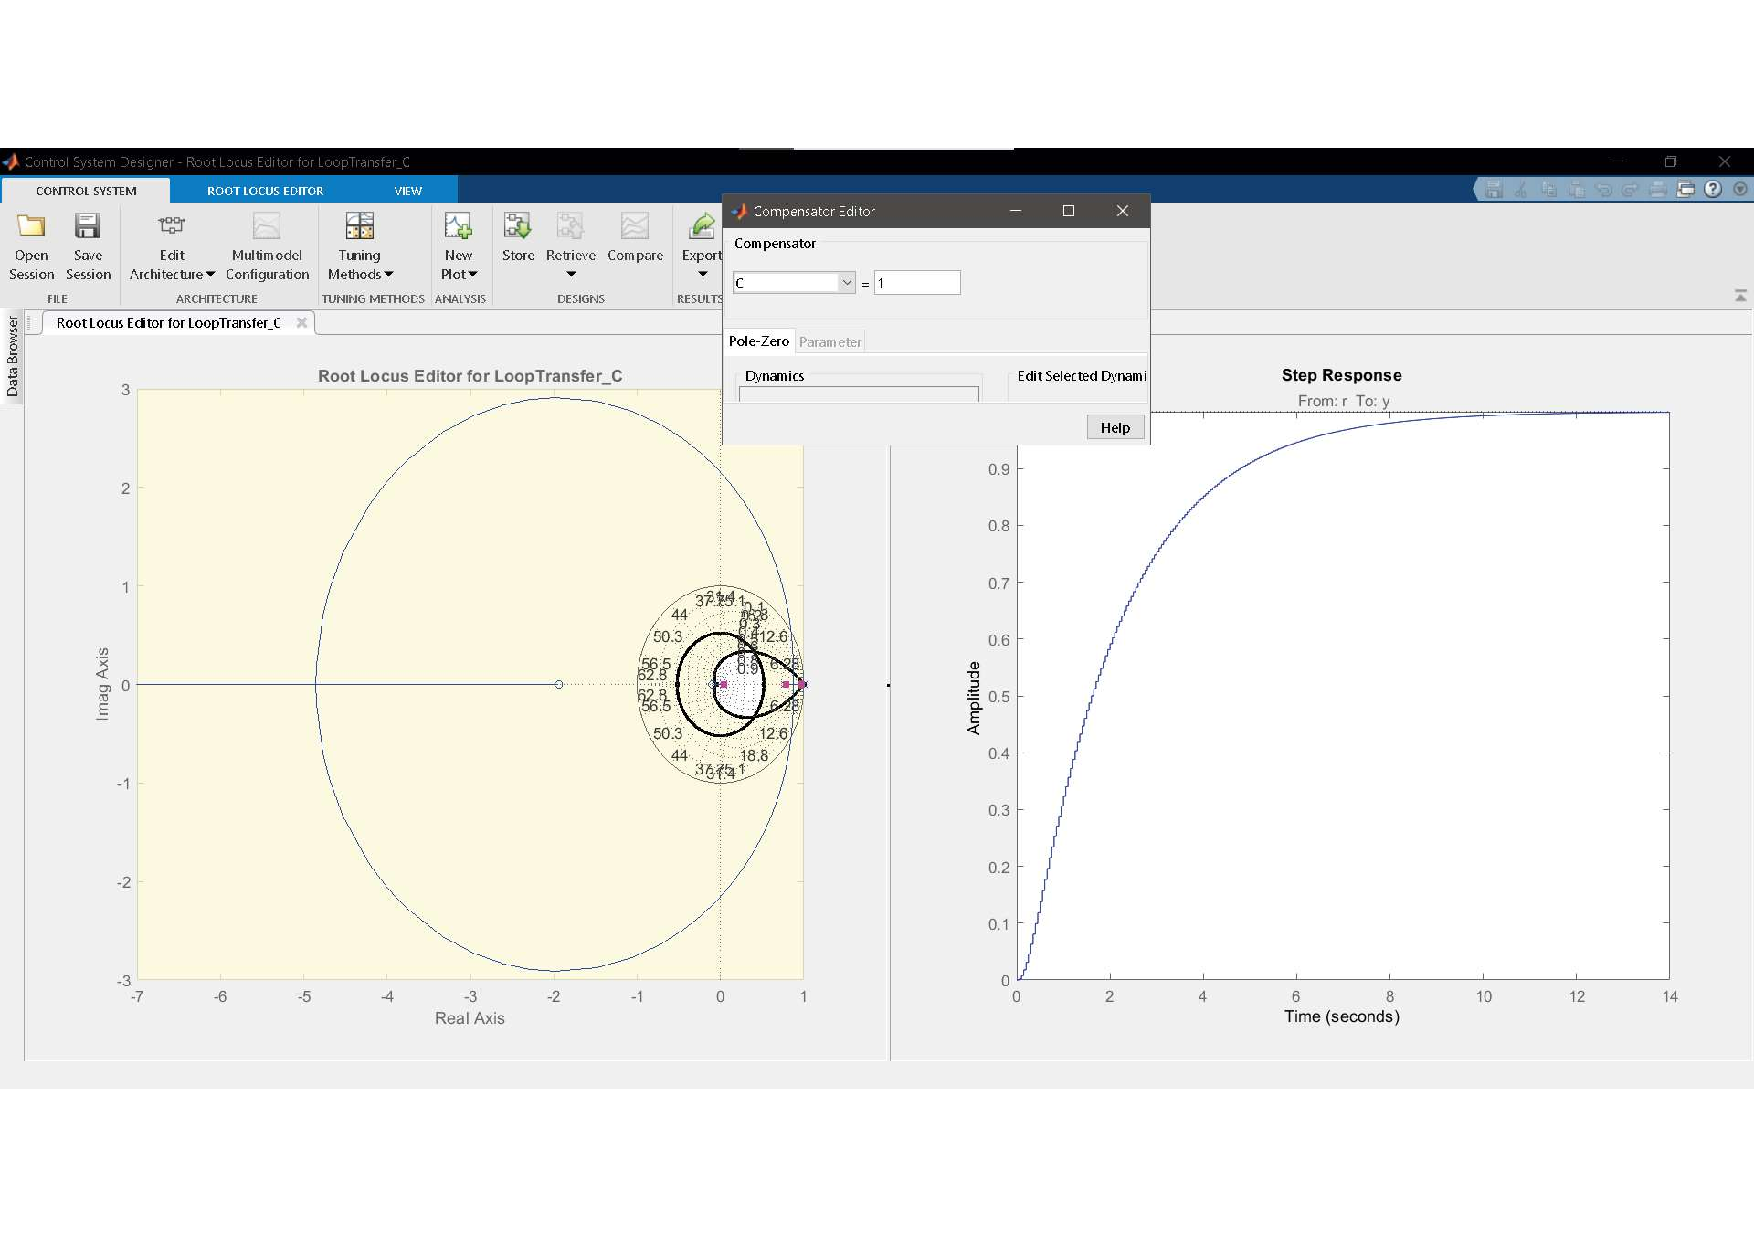
\includegraphics[clip, trim=0cm 3.5cm 0cm 2.4cm,scale=0.45]{images/figura 5.pdf}
  % izquierda,abajo,derecha,arriba
  \caption{Compensador proporcional con ganancia igual a 1.}
    \label{fig:figura 5}
\end{figure}
}

\end{tcolorbox}%

Utilizando el comando \textsc{rltool} con nuestra planta, en la
ventana \textsc{root locus editor} añadimos las especificaciones
necesarias, se puede observar como los polos en bucle cerrado en
nuestro lugar de la raices nunca llegan a cumplir todas las
especificaciones con un control proporcional ya que los polos en bucle
cerrado nunca llegan a la zona blanca sin importar la ganancia
positiva que pongamos.
